%Doc config

\documentclass[11pt,letterpaper]{article}
\setlength{\parindent}{0em}                  %Einrückungsabstand
\setlength{\parskip}{0.5em}                  %ABSTAND ZWISCHEN DEN ABSÄTZEN
\textwidth 6.5in
\textheight 9.in
\oddsidemargin 0in
\headheight 0in

%Module

\usepackage{fancybox}
\usepackage[utf8]{inputenc}
\usepackage{epsfig,graphicx}
\usepackage{multicol,pst-plot}
\usepackage{pstricks}
\usepackage{amsmath}
\usepackage{amsfonts}
\usepackage{amssymb}
\usepackage{eucal}
\usepackage[left=2cm,right=2cm,top=2cm,bottom=2cm]{geometry}
\usepackage{txfonts}
\usepackage[english]{babel}
\usepackage[colorlinks]{hyperref}
\usepackage{cancel}
\usepackage{caption}
\usepackage{float}
\usepackage{upgreek}
\usepackage{gensymb}
\usepackage{subfigure}
\usepackage{siunitx}
\usepackage{color}
\usepackage{tikz}
\usepackage{listings}
\usepackage{minted}
%\usepackage{mdframed}
\usepackage{natbib}
\bibliographystyle{mnras}
\setcitestyle{aysep{","}}
\usepackage{multicol}
\renewcommand{\bibpreamble}{\begin{multicols}{2}}
\renewcommand{\bibpostamble}{\end{multicols}}
\setlength{\bibsep}{3pt}

%colors

\definecolor{codegreen}{rgb}{0,0.6,0}
\definecolor{codegray}{rgb}{0.5,0.5,0.5}
\definecolor{backcolour}{rgb}{0.95,0.95,0.95}
\hypersetup{colorlinks=true,linkcolor=codegreen,citecolor=blue,filecolor=blue,urlcolor=magenta,}

%configuration listings

\lstset{ %
language=python,                % choose the language of the code
basicstyle=\footnotesize,       % the size of the fonts that are used for the code
numbers=left,                   % where to put the line-numbers
numberstyle=\footnotesize,      % the size of the fonts that are used for the line-numbers
stepnumber=1,                   % the step between two line-numbers. If it is 1 each line will be numbered
numbersep=5pt,                  % how far the line-numbers are from the code
backgroundcolor=\color{white},  % choose the background color. You must add \usepackage{color}
showspaces=false,               % show spaces adding particular underscores
showstringspaces=false,         % underline spaces within strings
showtabs=false,                 % show tabs within strings adding particular underscores
frame=single,                   % adds a frame around the code
tabsize=2,                      % sets default tabsize to 2 spaces
captionpos=b,                   % sets the caption-position to bottom
breaklines=true,                % sets automatic line breaking
breakatwhitespace=false,        % sets if automatic breaks should only happen at whitespace
escapeinside={\%*}{*)}          % if you want to add a comment within your code
}
\lstdefinestyle{mystyle}{
	backgroundcolor=\color{backcolour},   
	commentstyle=\color{red},
	keywordstyle=\bfseries\color{magenta},
	numberstyle=\tiny\color{codegray},
	stringstyle=\color{codegreen},
	basicstyle=\footnotesize\ttfamily,
	identifierstyle=\color{blue},
	breakatwhitespace=false,         
	breaklines=true,                 
	captionpos=b,                    
	keepspaces=true,                 
	numbers=left,                    
	numbersep=5pt,                  
	showspaces=false,                
	showstringspaces=false,
	showtabs=false,                  
	tabsize=2
}

\lstset{style=mystyle}

%configuration minted style

\usemintedstyle{vs}

%extra comands

\pagestyle{empty}
\DeclareMathOperator{\tr}{Tr}                      %ICONO TRAZA MECANICA CUANTICA
\DeclareMathOperator{\rsol}{R_\odot}               %ICONO RADIO SOLAR
\DeclareMathOperator{\lsol}{L_\odot}               %ICONO LUMINOSIDAD SOLAR
\DeclareMathOperator{\msol}{M_\odot}               %ICONO MASA SOLAR
\DeclareMathOperator{\probabi}{Prob}               %ICONO PROBABILIDAD
\newcommand{\units}[1]{\left[ #1 \right]}          %CORCHETES PARA UNIDADES
\newcommand{\prob}[1]{\probabi\left( #1 \right)}   %OPERADOR PROBABILIDAD
\newcommand{\abs}[1]{\left|#1\right|}              %OPERADOR VALOR ABSOLUTO
\newcommand{\bra}[1]{\langle #1 |}                 %OPERADOR BRA
\newcommand{\ket}[1]{| #1 \rangle}                 %OPERADOR KET
\newcommand{\braket}[2]{\langle #1 | #2 \rangle}   %OPERADOR BRA-KET
\newcommand{\ketbra}[2]{|#1\rangle\langle#2|}      %OPERADOR KET-BRA
\newcommand{\mean}[1]{\langle #1 \rangle}          %PROMEDIO MECANICA CUANTICA
\newcommand{\eval}[3]{\left.#1\right|_{#2}^{#3}}   %COMANDO PARA EVALUAR INTEGRALES

%DEFINICIÓN DE REVISTAS CIENTÍFICAS

\newcommand\aap{A\&A}                % Astronomy and Astrophysics
\let\astap=\aap                          % alternative shortcut
\newcommand\aapr{A\&ARv}             % Astronomy and Astrophysics Review (the)
\newcommand\aaps{A\&AS}              % Astronomy and Astrophysics Supplement Series
\newcommand\actaa{Acta Astron.}      % Acta Astronomica
\newcommand\afz{Afz}                 % Astrofizika
\newcommand\aj{AJ}                   % Astronomical Journal (the)
\newcommand\ao{Appl. Opt.}           % Applied Optics
\let\applopt=\ao                         % alternative shortcut
\newcommand\aplett{Astrophys.~Lett.} % Astrophysics Letters
\newcommand\apj{ApJ}                 % Astrophysical Journal
\newcommand\apjl{ApJ}                % Astrophysical Journal, Letters
\let\apjlett=\apjl                       % alternative shortcut
\newcommand\apjs{ApJS}               % Astrophysical Journal, Supplement
\let\apjsupp=\apjs                       % alternative shortcut
% The following journal does not appear to exist! Disabled.
%\newcommand\apspr{Astrophys.~Space~Phys.~Res.} % Astrophysics Space Physics Research
\newcommand\apss{Ap\&SS}             % Astrophysics and Space Science
\newcommand\araa{ARA\&A}             % Annual Review of Astronomy and Astrophysics
\newcommand\arep{Astron. Rep.}       % Astronomy Reports
\newcommand\aspc{ASP Conf. Ser.}     % ASP Conference Series
\newcommand\azh{Azh}                 % Astronomicheskii Zhurnal
\newcommand\baas{BAAS}               % Bulletin of the American Astronomical Society
\newcommand\bac{Bull. Astron. Inst. Czechoslovakia} % Bulletin of the Astronomical Institutes of Czechoslovakia 
\newcommand\bain{Bull. Astron. Inst. Netherlands} % Bulletin Astronomical Institute of the Netherlands
\newcommand\caa{Chinese Astron. Astrophys.} % Chinese Astronomy and Astrophysics
\newcommand\cjaa{Chinese J.~Astron. Astrophys.} % Chinese Journal of Astronomy and Astrophysics
\newcommand\fcp{Fundamentals Cosmic Phys.}  % Fundamentals of Cosmic Physics
\newcommand\gca{Geochimica Cosmochimica Acta}   % Geochimica Cosmochimica Acta
\newcommand\grl{Geophys. Res. Lett.} % Geophysics Research Letters
\newcommand\iaucirc{IAU~Circ.}       % IAU Cirulars
\newcommand\icarus{Icarus}           % Icarus
\newcommand\japa{J.~Astrophys. Astron.} % Journal of Astrophysics and Astronomy
\newcommand\jcap{J.~Cosmology Astropart. Phys.} % Journal of Cosmology and Astroparticle Physics
\newcommand\jcp{J.~Chem.~Phys.}      % Journal of Chemical Physics
\newcommand\jgr{J.~Geophys.~Res.}    % Journal of Geophysics Research
\newcommand\jqsrt{J.~Quant. Spectrosc. Radiative Transfer} % Journal of Quantitiative Spectroscopy and Radiative Transfer
\newcommand\jrasc{J.~R.~Astron. Soc. Canada} % Journal of the RAS of Canada
\newcommand\memras{Mem.~RAS}         % Memoirs of the RAS
\newcommand\memsai{Mem. Soc. Astron. Italiana} % Memoire della Societa Astronomica Italiana
\newcommand\mnassa{MNASSA}           % Monthly Notes of the Astronomical Society of Southern Africa
\newcommand\mnras{MNRAS}             % Monthly Notices of the Royal Astronomical Society
\newcommand\na{New~Astron.}          % New Astronomy
\newcommand\nar{New~Astron.~Rev.}    % New Astronomy Review
\newcommand\nat{Nature}              % Nature
\newcommand\nphysa{Nuclear Phys.~A}  % Nuclear Physics A
\newcommand\pra{Phys. Rev.~A}        % Physical Review A: General Physics
\newcommand\prb{Phys. Rev.~B}        % Physical Review B: Solid State
\newcommand\prc{Phys. Rev.~C}        % Physical Review C
\newcommand\prd{Phys. Rev.~D}        % Physical Review D
\newcommand\pre{Phys. Rev.~E}        % Physical Review E
\newcommand\prl{Phys. Rev.~Lett.}    % Physical Review Letters
\newcommand\pasa{Publ. Astron. Soc. Australia}  % Publications of the Astronomical Society of Australia
\newcommand\pasp{PASP}               % Publications of the Astronomical Society of the Pacific
\newcommand\pasj{PASJ}               % Publications of the Astronomical Society of Japan
\newcommand\physrep{Phys.~Rep.}      % Physics Reports
\newcommand\physscr{Phys.~Scr.}      % Physica Scripta
\newcommand\planss{Planet. Space~Sci.} % Planetary Space Science
\newcommand\procspie{Proc.~SPIE}     % Proceedings of the Society of Photo-Optical Instrumentation Engineers
\newcommand\rmxaa{Rev. Mex. Astron. Astrofis.} % Revista Mexicana de Astronomia y Astrofisica
\newcommand\qjras{QJRAS}             % Quarterly Journal of the RAS
\newcommand\sci{Science}             % Science
\newcommand\skytel{Sky \& Telesc.}   % Sky and Telescope
\newcommand\solphys{Sol.~Phys.}      % Solar Physics
\newcommand\sovast{Soviet~Ast.}      % Soviet Astronomy (aka Astronomy Reports)
\newcommand\ssr{Space Sci. Rev.}     % Space Science Reviews
\newcommand\zap{Z.~Astrophys.}       % Zeitschrift fuer Astrophysik

%COMIENZA EL DOCUMENTO

\begin{document}

%CONFIGURACIÓN DEL ENCABEZADO

\usetikzlibrary{positioning}
\tikzset{every picture/.style={line width=0.75pt}}    
\pagestyle{plain}
\begin{flushleft}
M.A. Management, Communication \& IT \hfill [MCI]\\
Department Management, Communication \& IT\\
\underline{Management Center Innsbruck}
\end{flushleft}

\begin{flushright}\vspace{-5mm}
\includegraphics[height=1.5cm]{logo-mci.png}
\end{flushright}
 
\begin{center}\vspace{-1cm}
\textbf{\large Homework: Digital Behavior}\\   %Title
Florian Bigelmaier\\                         %Name
\end{center}
\rule{\linewidth}{0.1mm}


%DESDE AQUÍ SE ESCRIBE TODO EL CONTENIDO

\begin{abstract}
    \noindent
    Esta template de \LaTeX viene preparada con muchos paquetes útiles, ya sea para escribir resoluciones matemáticas, importar imágenes, figuras, códigos, crear hipervínculos, signos matemáticos y mucho más. La he preparado durante mis últimos 2 años en la universidad, para poder entregar trabajos ordenados y completos. Ha sido probar muchos paquetes, ver errores, solucionarlos, editar y personalizar estilos hasta al fin encontrar algo que me guste y poder compartir con los demás para que puedan ocuparlo directamente o tener una base bien estructurada para poder crear sus propias templates, espero sea de utilidad para cualquiera que llegue hasta acá\footnote{Última edición: 27 de Agosto, 12:54}.
\end{abstract}
\subsection*{Versión 0.4.1}
Actualmente mantengo 2 versiones de esta misma template, y cada numero tiene su significado. El 0 es por que sigue siendo una versión \textbf{en edición}, en el momento que llegue a la versión 1 considerare que ya esta finalizada y tiene todo lo necesario. El 4 es por la edición, esta es la cuarta gran edición que he realizado. El 1 viene de la cantidad de columnas en la template, siendo esta la versión de 1 columna. Por lo que la versión 0.4.1 es la cuarta edición de una columna aún mantenida.
\subsection*{Comandos personalizados}

Hay par de comandos personalizados que están un poco más arriba en el código (pienso incluir varios), y que ayudan con operadores en mecánica cuántica, astronomía y cálculo.\par

Es cierto que algunos comandos vienen ya en otros paquetes, sin embargo, quería que esta template tuviera sólo lo necesario y no un exceso de comandos que jamás se usaran, por eso a medida que voy necesitando nuevos comandos, yo mismo los voy creando como comando personalizado. Aquí algunos ejemplos de operadores bra y ket de mecánica cuántica:
\begin{align*}
    \bra{-1}L_y\ket{-1} &= \bra{-1}\frac{-i\hbar}{\sqrt{2}}\ket{0} & \bra{-1}L_y\ket{0} &= \bra{-1}\frac{i\hbar}{\sqrt{2}}(\ket{-1} - \ket{1}) & \bra{-1}L_y\ket{1} &= \bra{-1}\frac{i\hbar}{\sqrt{2}}\ket{0}\\
     &= 0 & &= \frac{i\hbar}{\sqrt{2}} & &= 0\\
    \bra{0}L_y\ket{-1} &= \bra{0}\frac{-i\hbar}{\sqrt{2}}\ket{0} & \bra{0}L_y\ket{0} &= \bra{0}\frac{i\hbar}{\sqrt{2}}(\ket{-1} - \ket{1}) & \bra{0}L_y\ket{1} &= \bra{0}\frac{i\hbar}{\sqrt{2}}\ket{0}\\
     &= \frac{-i\hbar}{\sqrt{2}} & &= 0 & &= \frac{i\hbar}{\sqrt{2}}
\end{align*}
Ejemplos de comando unidad y unidades de medida astronómicas:
\begin{equation*}
    G = 4.3\times10^{-6}\units{\frac{Km^2Kpc}{s^2\msol}} \hspace{1cm} L = 2^{3.5} = 11.3 \units{\lsol}
\end{equation*}

Y finalmente ejemplos del comando probabilidad, valor absoluto y evaluar integral:
\begin{equation*}
    \begin{split}
        \prob{\ket{-1_y}} &= \abs{\braket{-1_y}{\psi}}^2\\
        &= \abs{\frac{1}{\sqrt{2+\gamma^2}}\frac{\sqrt{2} - \gamma}{\sqrt{2}}}^2\\
        &= \frac{1}{2+\gamma^2}\frac{2-2\sqrt{2}\gamma + \gamma^2}{2}\\
         \\
        \prob{\ket{1_y}} &= \abs{\braket{1_y}{\psi}}^2\\
        &= \abs{\frac{1}{\sqrt{2+\gamma^2}}\frac{\sqrt{2} + \gamma}{\sqrt{2}}}^2\\
        &= \frac{1}{2+\gamma^2}\frac{2+2\sqrt{2}\gamma + \gamma^2}{2}
    \end{split}
    \qquad
    \begin{split}
        B(y_0) &= \frac{I\mu_0}{4\pi}\int_{-\frac{L}{2}}^{\frac{L}{2}} \frac{dz\hat{k}\times(y_0\hat{\jmath} - z\hat{k})}{(y_0^2 + z^2)^{\frac{3}{2}}}\\
        &= -\frac{I\mu_0}{4\pi}\int_{-\frac{L}{2}}^{\frac{L}{2}} \frac{y_0}{(y_0^2 + z^2)^{\frac{3}{2}}}dz\hat{\imath}\\
        &= -\frac{I\mu_0}{4\pi}\eval{\frac{z}{y_0\sqrt{z^2+y_0^2}}}{-\frac{L}{2}}{\frac{L}{2}}\hat{\imath}\\
        B(y_0) &= -\frac{I\mu_0}{2\pi y_0}\frac{L}{\sqrt{L^2 + 4y_0^2}}\hat{\imath}
    \end{split}
\end{equation*}

\subsection*{TikZ}
Un paquete muy potente es TikZ, que permite crear gráficos útiles (y bonitos) que ayudan al entendimiento del problema que se esta resolviendo. Muchas veces pasa que intentamos dibujar un gráfico en otro programa y no queda como queremos, o que directamente no sabemos como hacerlo y terminamos 'robando' una imagen X de Google, con esta herramienta eso ya no pasa, ya que es muy simple de usar y no desentona en el aspecto sobrio de \LaTeX.\par
Recomiendo \href{https://www.mathcha.io/}{Mathcha} para realizar buenos gráficos sin necesidad de saber escribir en TikZ, como por ejemplo:
\begin{figure}[H]
    \centering
    \begin{tikzpicture}[x=0.75pt,y=0.75pt,yscale=-1,xscale=1]
%uncomment if require: \path (0,300); %set diagram left start at 0, and has height of 300

%Shape: Axis 2D [id:dp8886271678946946] 
\draw [color={rgb, 255:red, 155; green, 155; blue, 155 }  ,draw opacity=1 ] (179.83,128.5) -- (279.83,128.5)(179.83,28.5) -- (179.83,128.5) -- cycle (272.83,123.5) -- (279.83,128.5) -- (272.83,133.5) (174.83,35.5) -- (179.83,28.5) -- (184.83,35.5)  ;
%Straight Lines [id:da7444971400775593] 
\draw [color={rgb, 255:red, 155; green, 155; blue, 155 }  ,draw opacity=1 ]   (179.83,128.5) -- (109.84,189.68) ;
\draw [shift={(108.33,191)}, rotate = 318.84000000000003] [color={rgb, 255:red, 155; green, 155; blue, 155 }  ,draw opacity=1 ][line width=0.75]    (10.93,-4.9) .. controls (6.95,-2.3) and (3.31,-0.67) .. (0,0) .. controls (3.31,0.67) and (6.95,2.3) .. (10.93,4.9)   ;
%Shape: Ellipse [id:dp8867278988090774] 
\draw  [color={rgb, 255:red, 155; green, 155; blue, 155 }  ,draw opacity=1 ][dash pattern={on 0.84pt off 2.51pt}] (114.33,128.5) .. controls (114.33,113.11) and (143.66,100.62) .. (179.83,100.62) .. controls (216.01,100.62) and (245.33,113.11) .. (245.33,128.5) .. controls (245.33,143.89) and (216.01,156.37) .. (179.83,156.37) .. controls (143.66,156.37) and (114.33,143.89) .. (114.33,128.5) -- cycle ;
%Straight Lines [id:da16420107689735763] 
\draw    (179.83,128.5) -- (151,154.33) ;
%Straight Lines [id:da00432643670206212] 
\draw    (179.83,128.5) -- (179.93,35.2) ;
\draw [shift={(179.93,33.2)}, rotate = 450.06] [color={rgb, 255:red, 0; green, 0; blue, 0 }  ][line width=0.75]    (10.93,-3.29) .. controls (6.95,-1.4) and (3.31,-0.3) .. (0,0) .. controls (3.31,0.3) and (6.95,1.4) .. (10.93,3.29)   ;
%Straight Lines [id:da33823555592256604] 
\draw    (179.83,128.5) -- (222.67,100) ;
\draw [shift={(222.67,100)}, rotate = 371.36] [color={rgb, 255:red, 0; green, 0; blue, 0 }  ][line width=0.75]    (-5.59,0) -- (5.59,0)(0,5.59) -- (0,-5.59)   ;
%Shape: Circle [id:dp8994173639458711] 
\draw   (114.33,128.5) .. controls (114.33,92.33) and (143.66,63) .. (179.83,63) .. controls (216.01,63) and (245.33,92.33) .. (245.33,128.5) .. controls (245.33,164.67) and (216.01,194) .. (179.83,194) .. controls (143.66,194) and (114.33,164.67) .. (114.33,128.5) -- cycle ;
%Straight Lines [id:da5294053812138602] 
\draw [color={rgb, 255:red, 155; green, 155; blue, 155 }  ,draw opacity=1 ] [dash pattern={on 4.5pt off 4.5pt}]  (179.88,80.85) -- (150.32,104.52) ;
%Straight Lines [id:da5842350667070813] 
\draw [color={rgb, 255:red, 155; green, 155; blue, 155 }  ,draw opacity=1 ] [dash pattern={on 4.5pt off 4.5pt}]  (151,154.33) -- (150.32,104.52) ;
%Straight Lines [id:da2647858047247953] 
\draw    (179.83,128.5) -- (91.88,56.27) ;
\draw [shift={(90.33,55)}, rotate = 399.39] [color={rgb, 255:red, 0; green, 0; blue, 0 }  ][line width=0.75]    (10.93,-3.29) .. controls (6.95,-1.4) and (3.31,-0.3) .. (0,0) .. controls (3.31,0.3) and (6.95,1.4) .. (10.93,3.29)   ;
%Shape: Arc [id:dp1170495504919975] 
\draw  [draw opacity=0] (160.72,112.93) .. controls (166.32,108.12) and (172.86,104.45) .. (180,102.26) -- (195.55,157.02) -- cycle ; \draw   (160.72,112.93) .. controls (166.32,108.12) and (172.86,104.45) .. (180,102.26) ;
%Shape: Arc [id:dp4167292362856063] 
\draw  [draw opacity=0] (179.72,102.36) .. controls (187.39,105.12) and (194.33,109.18) .. (200.18,114.23) -- (155.95,155.36) -- cycle ; \draw   (179.72,102.36) .. controls (187.39,105.12) and (194.33,109.18) .. (200.18,114.23) ;

%Shape: Axis 2D [id:dp6964913109306807] 
\draw [color={rgb, 255:red, 155; green, 155; blue, 155 }  ,draw opacity=1 ] (470.83,129.83) -- (570.83,129.83)(470.83,29.83) -- (470.83,129.83) -- cycle (563.83,124.83) -- (570.83,129.83) -- (563.83,134.83) (465.83,36.83) -- (470.83,29.83) -- (475.83,36.83)  ;
%Straight Lines [id:da9799737640979158] 
\draw [color={rgb, 255:red, 155; green, 155; blue, 155 }  ,draw opacity=1 ]   (470.83,129.83) -- (400.84,191.02) ;
\draw [shift={(399.33,192.33)}, rotate = 318.84000000000003] [color={rgb, 255:red, 155; green, 155; blue, 155 }  ,draw opacity=1 ][line width=0.75]    (10.93,-4.9) .. controls (6.95,-2.3) and (3.31,-0.67) .. (0,0) .. controls (3.31,0.67) and (6.95,2.3) .. (10.93,4.9)   ;
%Shape: Ellipse [id:dp26582670799657215] 
\draw  [color={rgb, 255:red, 155; green, 155; blue, 155 }  ,draw opacity=1 ][dash pattern={on 0.84pt off 2.51pt}] (405.33,129.83) .. controls (405.33,114.44) and (434.66,101.96) .. (470.83,101.96) .. controls (507.01,101.96) and (536.33,114.44) .. (536.33,129.83) .. controls (536.33,145.23) and (507.01,157.71) .. (470.83,157.71) .. controls (434.66,157.71) and (405.33,145.23) .. (405.33,129.83) -- cycle ;
%Straight Lines [id:da7544277310094294] 
\draw    (470.83,129.83) -- (442,155.67) ;
%Straight Lines [id:da1285374936569712] 
\draw    (470.83,129.83) -- (470.93,36.53) ;
\draw [shift={(470.93,34.53)}, rotate = 450.06] [color={rgb, 255:red, 0; green, 0; blue, 0 }  ][line width=0.75]    (10.93,-3.29) .. controls (6.95,-1.4) and (3.31,-0.3) .. (0,0) .. controls (3.31,0.3) and (6.95,1.4) .. (10.93,3.29)   ;
%Straight Lines [id:da25141353979627534] 
\draw    (470.83,129.83) -- (513.67,101.33) ;
\draw [shift={(513.67,101.33)}, rotate = 371.36] [color={rgb, 255:red, 0; green, 0; blue, 0 }  ][line width=0.75]    (-5.59,0) -- (5.59,0)(0,5.59) -- (0,-5.59)   ;
%Shape: Circle [id:dp3725802003649237] 
\draw   (405.33,129.83) .. controls (405.33,93.66) and (434.66,64.33) .. (470.83,64.33) .. controls (507.01,64.33) and (536.33,93.66) .. (536.33,129.83) .. controls (536.33,166.01) and (507.01,195.33) .. (470.83,195.33) .. controls (434.66,195.33) and (405.33,166.01) .. (405.33,129.83) -- cycle ;
%Straight Lines [id:da7372964779325462] 
\draw    (470.83,129.83) -- (382.88,57.6) ;
\draw [shift={(381.33,56.33)}, rotate = 399.39] [color={rgb, 255:red, 0; green, 0; blue, 0 }  ][line width=0.75]    (10.93,-3.29) .. controls (6.95,-1.4) and (3.31,-0.3) .. (0,0) .. controls (3.31,0.3) and (6.95,1.4) .. (10.93,3.29)   ;
%Shape: Arc [id:dp05119912756037448] 
\draw  [draw opacity=0] (451.72,114.26) .. controls (457.32,109.46) and (463.86,105.79) .. (471,103.59) -- (486.55,158.36) -- cycle ; \draw   (451.72,114.26) .. controls (457.32,109.46) and (463.86,105.79) .. (471,103.59) ;


% Text Node
\draw (169,224) node [anchor=north west][inner sep=0.75pt]   [align=left] {(a)};
% Text Node
\draw (459.33,221.67) node [anchor=north west][inner sep=0.75pt]   [align=left] {(b)};
% Text Node
\draw (190,163.33) node [anchor=north west][inner sep=0.75pt]   [align=left] {$\displaystyle \sigma $};
% Text Node
\draw (155.33,123.67) node [anchor=north west][inner sep=0.75pt]   [align=left] {$\displaystyle a$};
% Text Node
\draw (169.33,109.33) node [anchor=north west][inner sep=0.75pt]  [font=\scriptsize] [align=left] {$\displaystyle \alpha $};
% Text Node
\draw (180.84,111.79) node [anchor=north west][inner sep=0.75pt]  [font=\scriptsize,rotate=-359.87] [align=left] {$\displaystyle \theta '$};
% Text Node
\draw (105.33,46.33) node [anchor=north west][inner sep=0.75pt]   [align=left] {$\displaystyle \omega $};
% Text Node
\draw (182,43) node [anchor=north west][inner sep=0.75pt]   [align=left] {$\displaystyle r$};
% Text Node
\draw (203.67,110.33) node [anchor=north west][inner sep=0.75pt]   [align=left] {$\displaystyle r'$};
% Text Node
\draw (124,176) node [anchor=north west][inner sep=0.75pt]   [align=left] {x};
% Text Node
\draw (258.33,129) node [anchor=north west][inner sep=0.75pt]   [align=left] {y};
% Text Node
\draw (161.67,23.67) node [anchor=north west][inner sep=0.75pt]   [align=left] {z};
% Text Node
\draw (481,164.67) node [anchor=north west][inner sep=0.75pt]   [align=left] {$\displaystyle \sigma $};
% Text Node
\draw (446.33,125) node [anchor=north west][inner sep=0.75pt]   [align=left] {$\displaystyle a$};
% Text Node
\draw (460.33,110.67) node [anchor=north west][inner sep=0.75pt]  [font=\scriptsize] [align=left] {$\displaystyle \theta $};

% Text Node
\draw (474,44) node [anchor=north west][inner sep=0.75pt]   [align=left] {$\displaystyle \omega $};
% Text Node
\draw (401,50.67) node [anchor=north west][inner sep=0.75pt]   [align=left] {$\displaystyle r$};
% Text Node
\draw (494.67,111.67) node [anchor=north west][inner sep=0.75pt]   [align=left] {$\displaystyle r'$};
% Text Node
\draw (415,177.33) node [anchor=north west][inner sep=0.75pt]   [align=left] {x};
% Text Node
\draw (549.33,130.33) node [anchor=north west][inner sep=0.75pt]   [align=left] {y};
% Text Node
\draw (452.67,25) node [anchor=north west][inner sep=0.75pt]   [align=left] {z};


\end{tikzpicture}
    \caption{Gráfico esquemático creado con Mathcha y exportado en formato TikZ.}
    \label{fig:1}
\end{figure}
\newpage
\subsection*{Imprimir códigos de programación}
Siempre resultara útil poder escribir el código que uno uso para poder realizar cálculos o gráficos, y si bien, es mucho mejor enviar el código como un archivo a parte, aveces tener una previsualización en el informe basta y sobra. Para esto se tienen dos módulos muy similares, elige el que más te guste para usar.\par
Es posible imprimir código con el paquete \textbf{lstlistings}:
\lstinputlisting{code.py}
También es posible con el paquete \textbf{Minted}:
\begin{mdframed}[backgroundcolor=backcolour]
    \inputminted[]{python}{code.py}
\end{mdframed}

Cabe destacar que estos paquetes no reconocen tildes, comillas dobles o cualquier carácter fuera del formato UTF-8, por lo que hay que tener cuidado, ya que puede producir errores o directamente no compilar el pdf.
\subsection*{Incluir imágenes}

Esto es un clásico de las tareas e informes, siempre una buena imagen (como esta \ref{code1}) deja más claro el resultado de un ejercicio o es un paso fundamental de lo que se esta pidiendo. En este caso incluyo la imagen resultante al compilar el código de antes:
\begin{figure}[H]
        \centering
        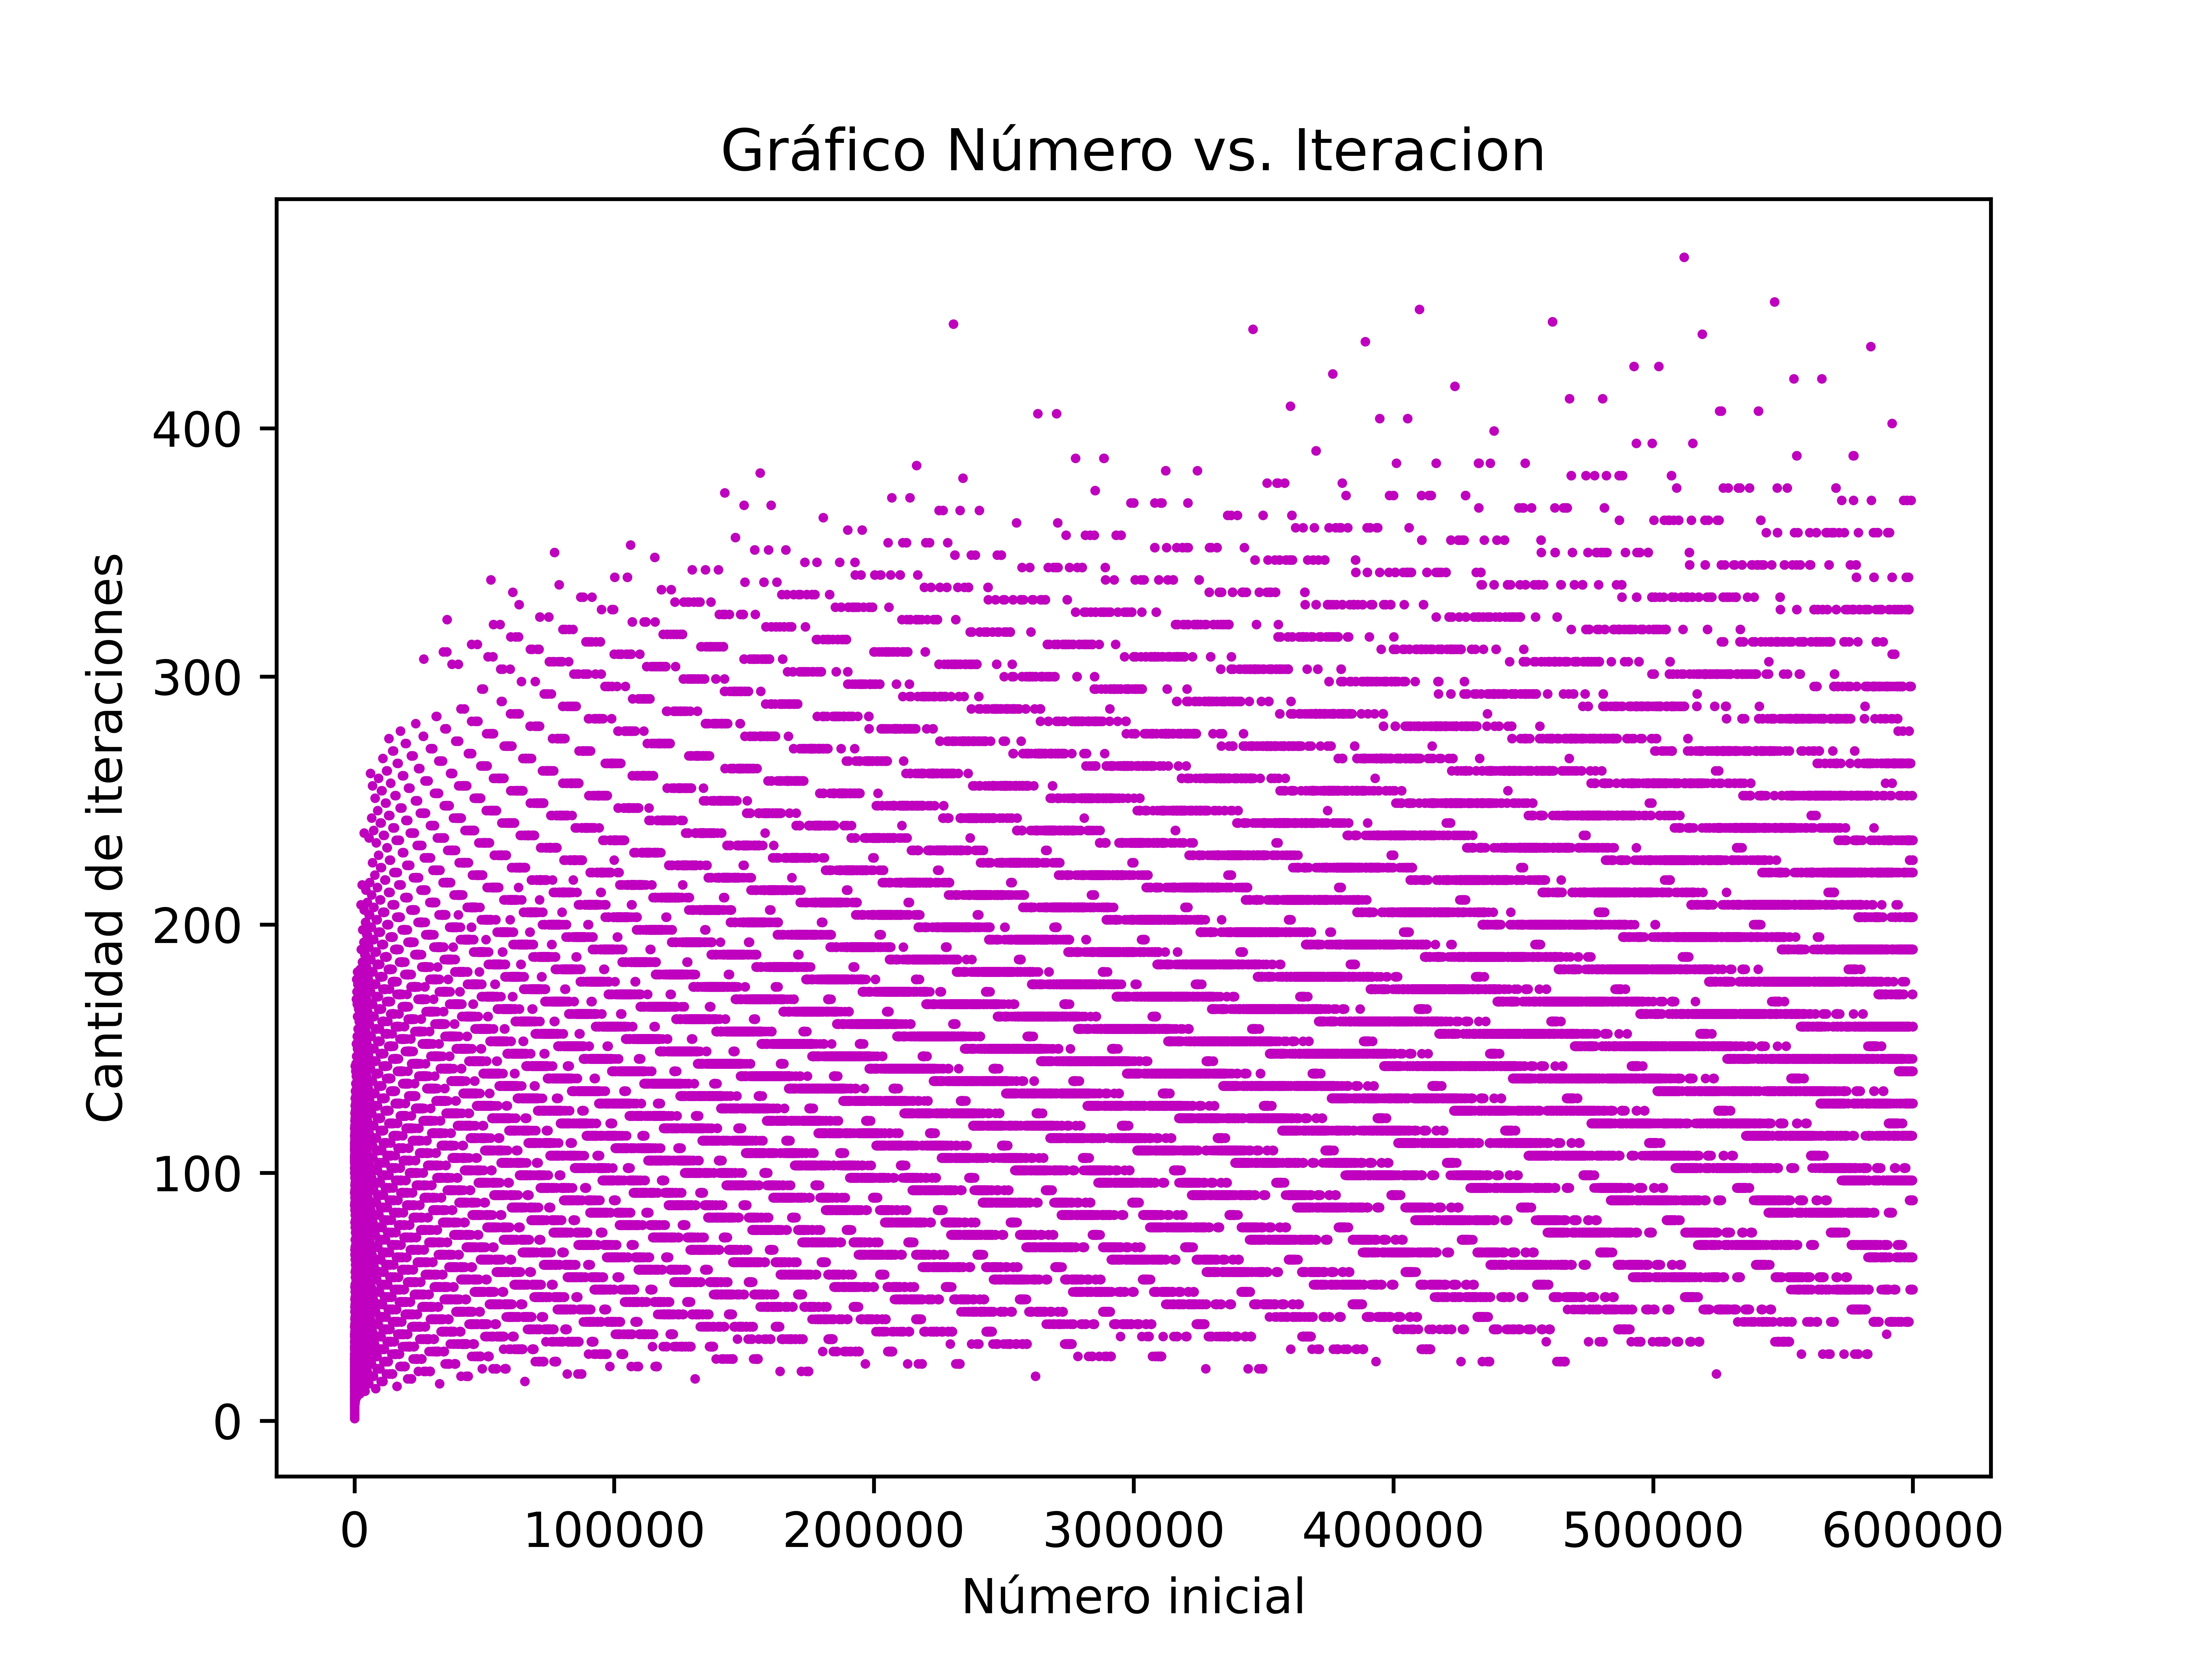
\includegraphics[]{foto.png}
        \caption{Imagen resultante del código para la Conjetura de Collatz cuando se ingresa un input de $x=600000$.}
        \label{code1}
\end{figure}
\subsection*{Bibliografía y Referencias}
Esta template hace uso del paquete \textbf{natbib} para administrar de manera sencilla las referencias usadas en el informe, para ello se debe de obtener la referencia en formato \textbf{BibTex}, pegarla en el archivo \textbf{biblio.bib} y luego citar de manera correcta en el texto. Abajo se incluye un texto de ejemplo con varias referencias correctamente utilizadas. El estilo utilizado pertenece a la Monthly Notices of the Royal Astronomical Society (MNRAS), sin embargo todos los parámetros son editables, ya sea en el preámbulo del contenido en este archivo \textbf{.tex} o en el archivo de estilo bibliográfico \textbf{mnras.bst}.

\subsection*{Texto de ejemplo}
La teoría de la Relatividad General de \cite{Einstein1915} predecía la existencia de objetos infinitamente densos cuya atracción gravitatoria era tan extrema, que ni la misma luz podía escapar de ella \citep{Schwarzschild_2003}, esto hace ya más de 100 años, tiempo en el cual se han realizado múltiples investigaciones para probar esta predicción. En un principio se dudaba de que esto fuera un hecho como tal, y que sólo suponía una solución a un problema matemático y que algún mecanismo evitaría la creación de estos objetos, sin embargo, desarrollos teóricos referentes a colapsos gravitatorios presentaban escenarios donde era factible que esto ocurriera \citep{10.1093/mnras/91.5.456} y tan sólo unos años después se pudo presentar una descripción teórica completa para estrellas supermasivas sin momento angular que ante el cese de reacciones nucleares, colapsarían ante la gravedad, la cual superaría a las fuerzas fundamentales y terminaría por producir el agujero negro (BH) predicho por Schwarzschild \citep{PhysRev.56.455}. Múltiples descripciones para casos rotacionales \citep{PhysRevLett.11.237}, cargados eléctricamente \citep{newman1965metric} y estacionarios \citep{israel1967event} se presentaron con el pasar de los años, y el más importante fue sin lugar a dudas el trabajo realizado por \cite{PhysRevLett.14.57} quien logro demostrar que si la Relatividad General era correcta, los agujeros negros deberían de existir, por lo que el marco teórico que respaldaba la existencia de estos objetos era bastante firme.\\
Observaciones y posteriores estudios realizados por \cite{1970ApJ...161..419W} presentaban fuertes argumentos a favor de la existencia de los agujeros negros, puesto que eran necesarios para la formación de galaxias elípticas dadas las cantidades masivas de materia presentes en el núcleo de las mismas. Esta idea tomo fuerza luego de que se observaran diferencias notorias de la dinámica estelar entre las zonas centrales y externas de la galaxia M87, lo que apuntaba seriamente a la presencia de un agujero negro supermasivo (SMBH) en el núcleo de la misma \citep{sargent1978dynamical}.\\
Muchos años antes, \cite{jansky1933electrical} realizo un estudio eléctrico en la atmósfera terrestre a longitudes de onda ($\lambda$) pertenecientes al radio, encontrándose con ciertas señales que no eran atribuibles a ninguna emisión terrestre, por lo que proponía que estas eran de origen interestelar, sin poder descifrar de donde provenían las señales detectadas. Estudios de radio en años posteriores estuvieron muy cerca de descubrir el origen \citep{clark, minley} y ya proponían la presencia de estructuras compactas en el GC haciendo analogía con quásares, dado que ya se habían observado fenómenos de alta energía en el CG \citep{lynden, lyndenress}. Unos pocos años después fue que \cite{balick1974intense} detectaron señales de radio muy potentes con el uso de interferometría en el National Radio Astronomy Observatory (NRAO) a $\lambda$ de $11\;\text{cm}$ y $3\;\text{cm}$ con resoluciones de $0.7''$ y $0.3''$ respectivamente (criterios que no se habían investigado anteriormente), que provenían del GC y que no se comparaban con registros anteriores, siendo este uno de los descubrimientos más importantes en radio astronomía de los años 70. Exactamente un año después, \cite{lo1} pudieron confirmar la detección con el uso de VLBI (Very Long Baseline Interferometry). Finalmente se termino adoptando el nombre de Sagitario A$^*$ (Sgr A$^*$ de aquí en adelante) para referirse a este SMBH en el GC \citep{brownestrella}.\\
En años recientes nace el Event Horizon Telescope (EHT) con la idea de obtener la primera imagen de un BH bajo la idea de que que éste debería de aparentar un mayor tamaño gracias a la deformación gravitacional \citep{campbell}. Los principales objetivos a observar eran los GCs de M87 (M87$^*$) y nuestra galaxia (Sgr A$^*$) que presentaban grandes posibilidades de albergar un SMBH. Las observaciones ya entregaron resultados para M87$^*$ \citep{2019ApJ...875L...2E}, presentando la primera imagen jamás obtenida de un SMBH.

\newpage
\bibliography{biblio}






\end{document}
